\section{Decay schemes of the studied sources}
\label{sec:decay_schemes}
%
\begin{figure}[htbp]
    \begin{minipage}[t]{0.5\textwidth}
        \centering
        \captionsetup{width=.95\linewidth}
        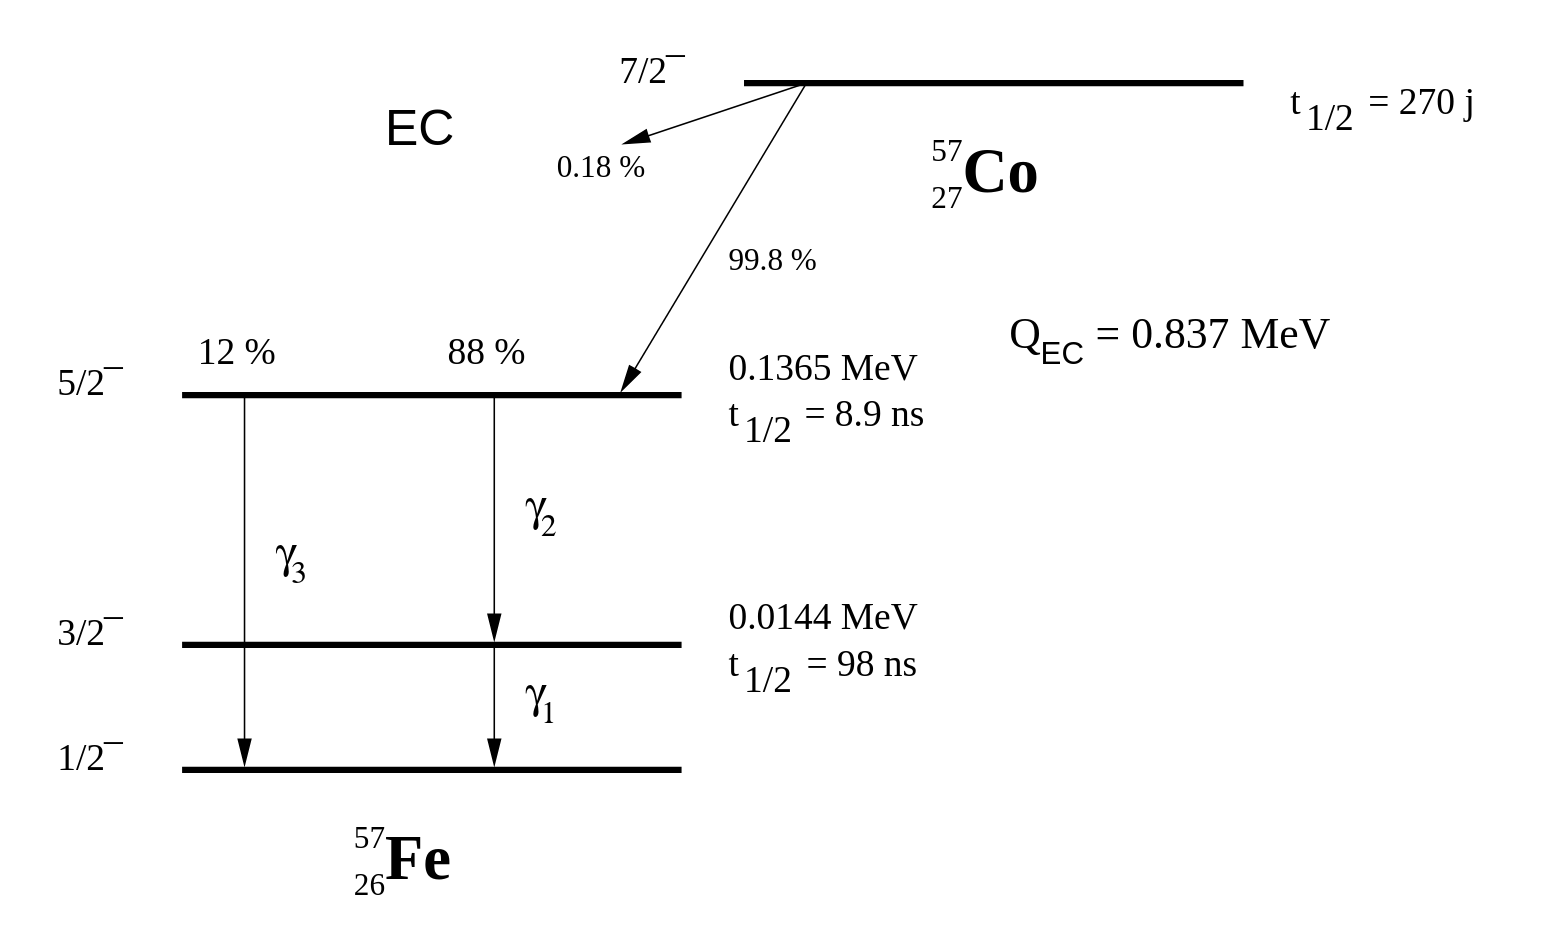
\includegraphics[width=\textwidth]{figures/decay_cobalt57.png}
        \caption{Decay scheme of \cobalt \cite{notice_VI}}
        \label{fig:cobalt_decay}
    \end{minipage}
    %
    \begin{minipage}[t]{0.5\textwidth}
        \centering
        \captionsetup{width=.95\linewidth}
        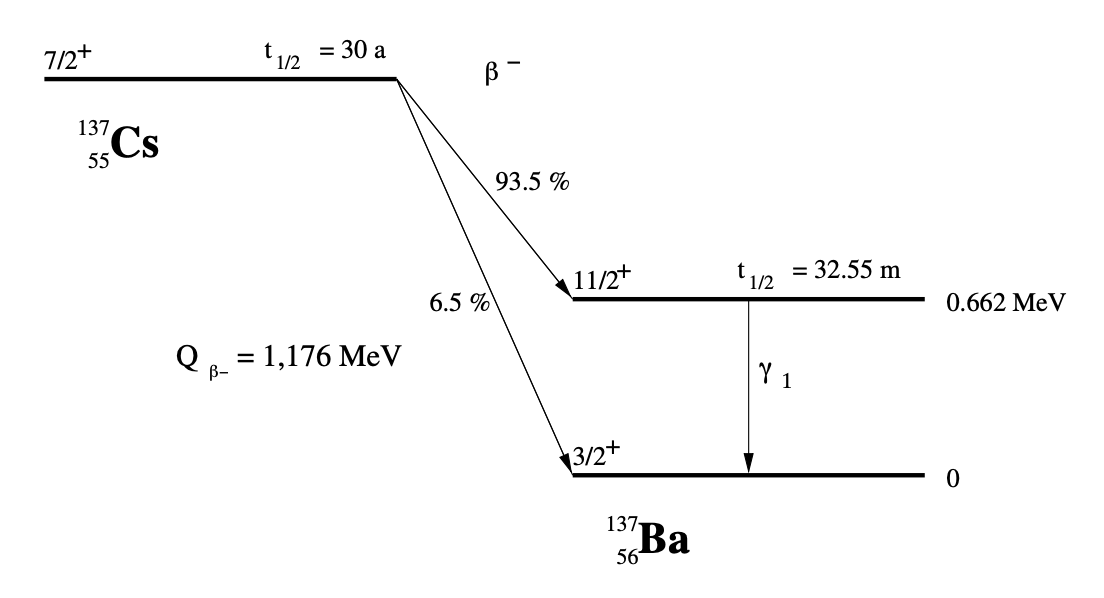
\includegraphics[width=\textwidth]{figures/decay_cesium137.png}
        \caption{Decay scheme of \cesium \cite{notice_VI}}
        \label{fig:cesium_decay}
    \end{minipage}
\end{figure}
%
\begin{figure}[htbp]
    \begin{minipage}[t]{0.5\textwidth}
        \centering
        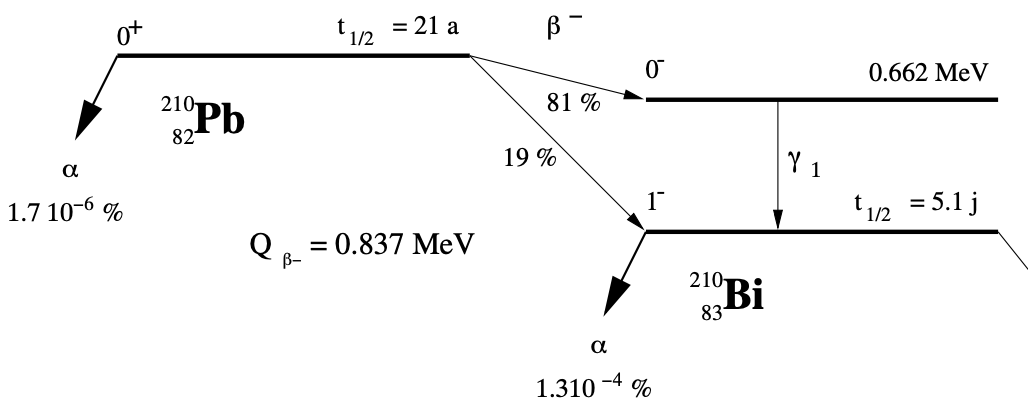
\includegraphics[width=1\textwidth]{figures/decay_lead210.png}
        \caption{Decay scheme of \lead \cite{notice_VI}}
        \label{fig:lead_decay}
    \end{minipage}
    \begin{minipage}[t]{0.5\textwidth}
        \centering
        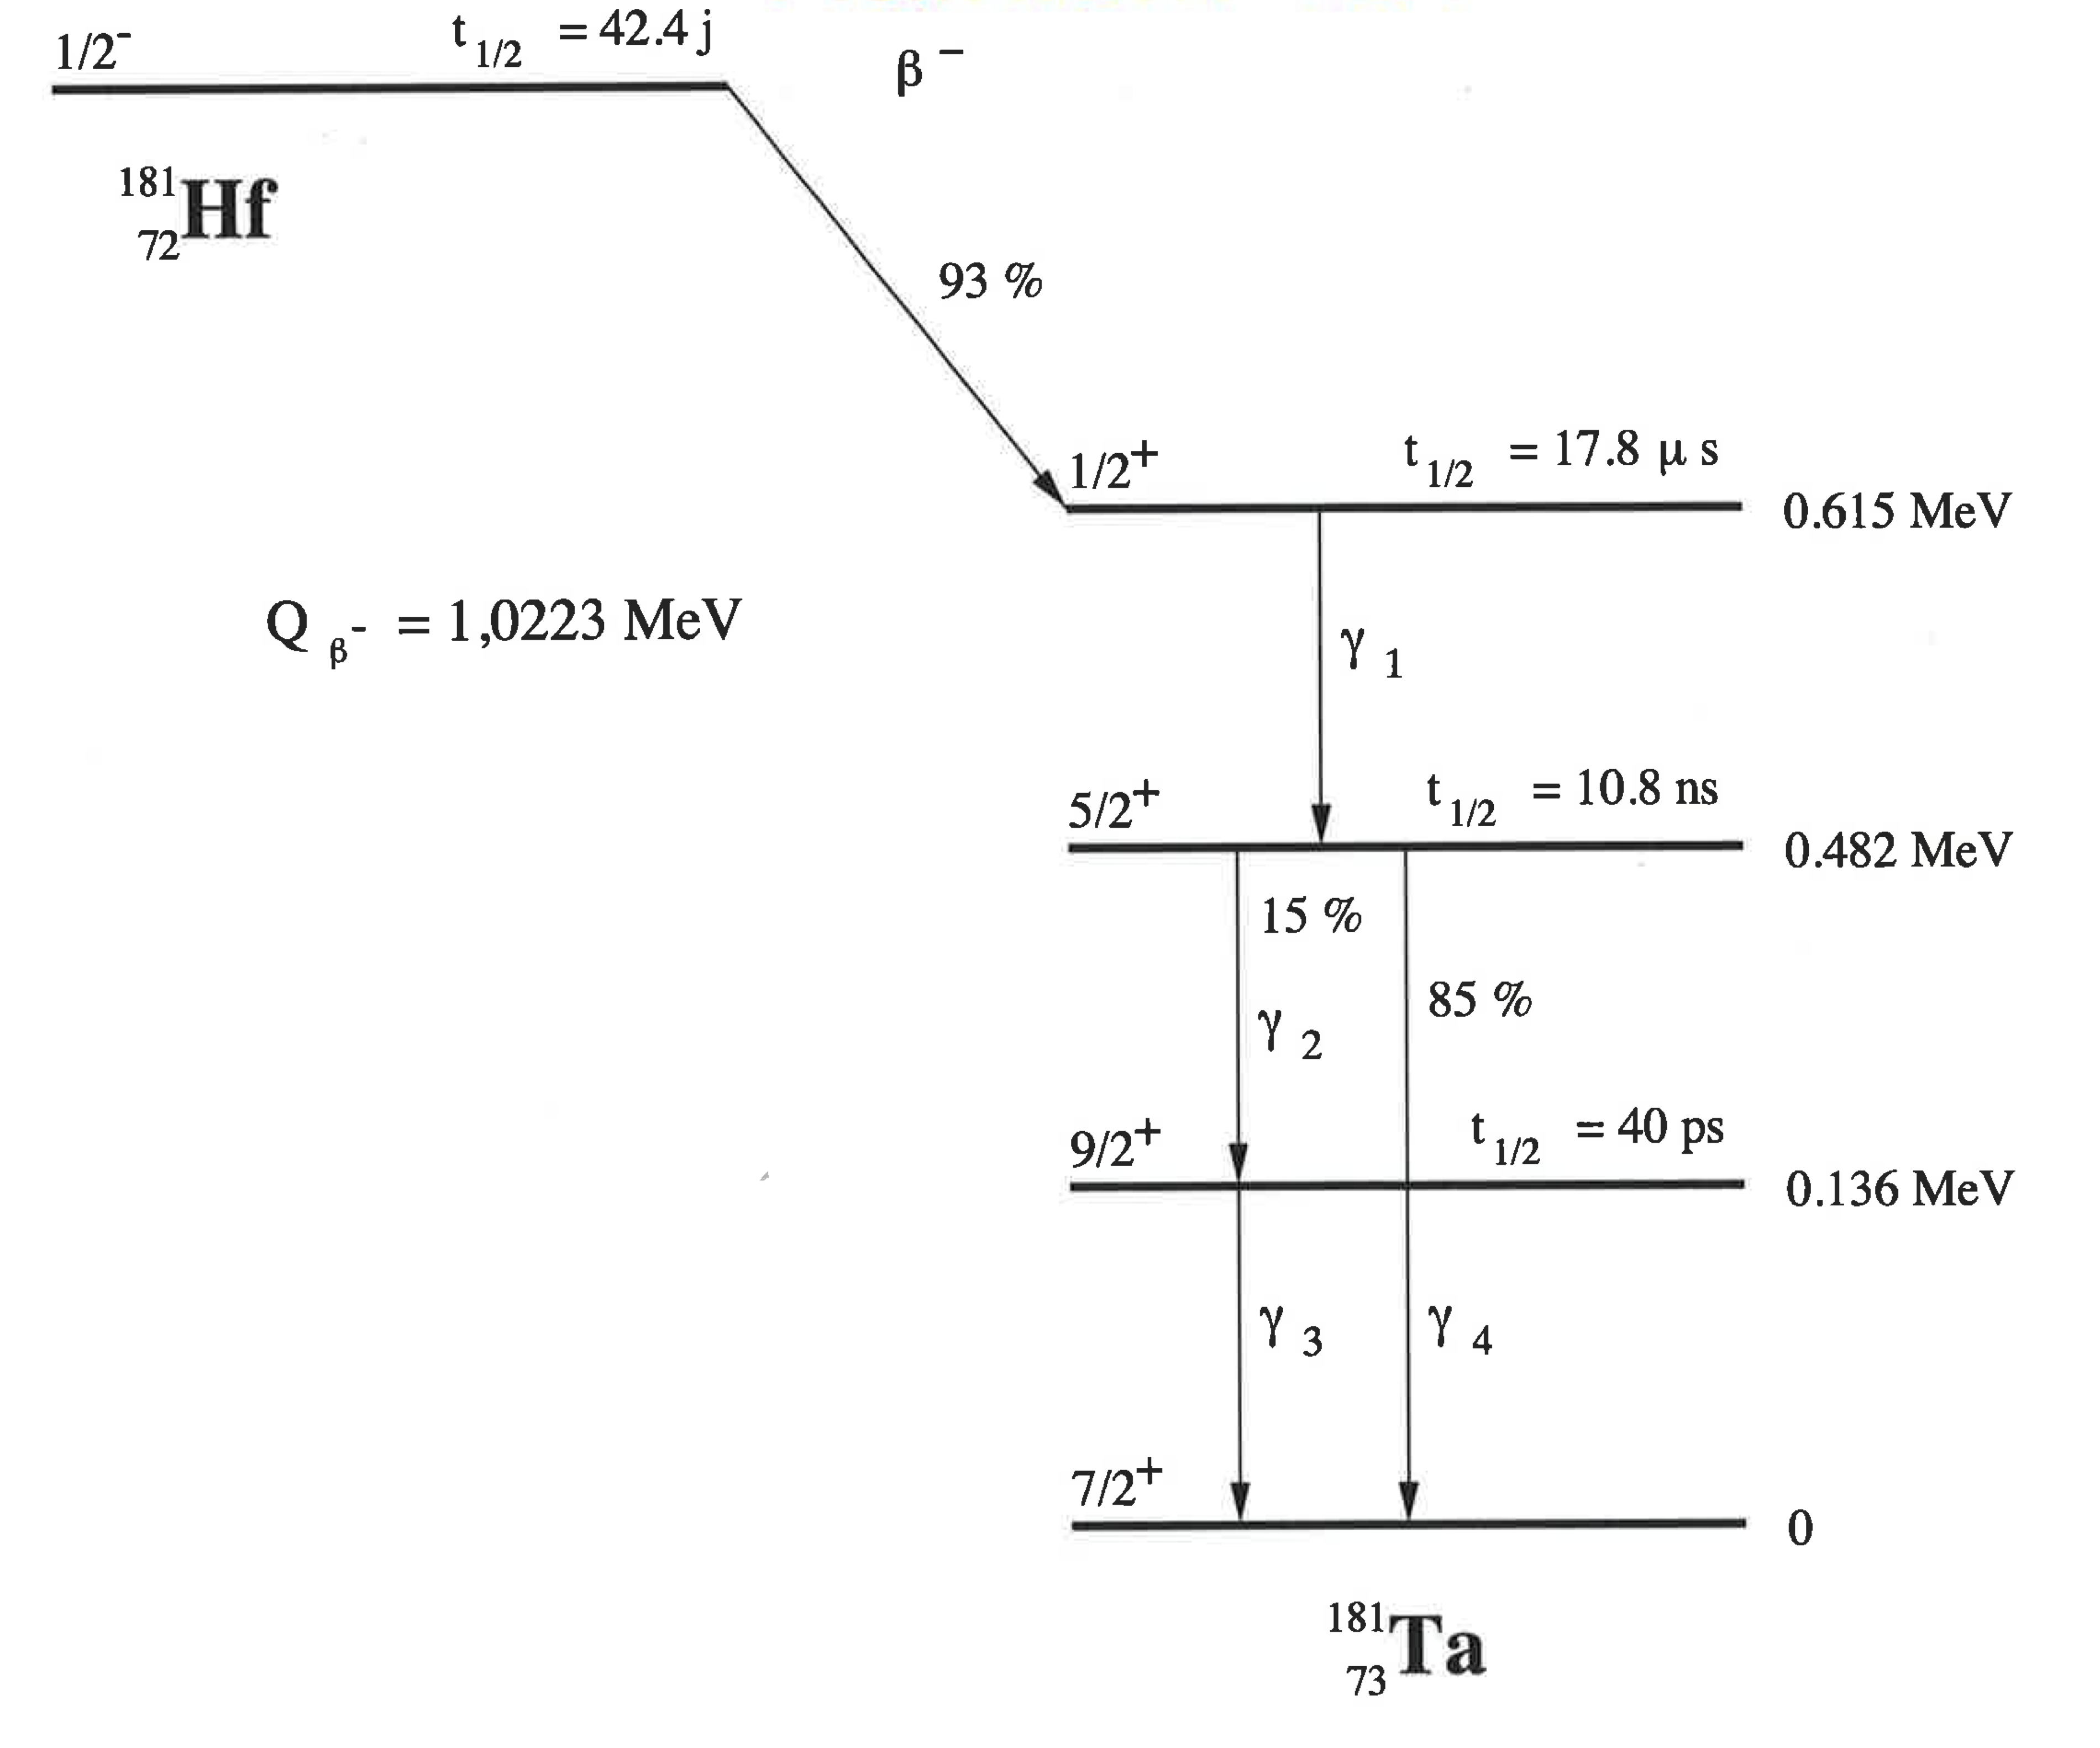
\includegraphics[width=\textwidth]{figures/decay_hafnium181.png}
        \caption{Decay scheme of \hafnium \cite{notice_VI}}
        \label{fig:hafnium_decay}
    \end{minipage}
\end{figure}

\section{Probabilities}
\label{sec:pearson}

\paragraph{Pearson's \(\chi^2\) test}
Let \(H0\) be the null-hypothesis "\(X \sim F\)", for some random variable \(X\) and some test distribution \(F\). Fix a number of samples \(N\).
The test statistic \(t\) is then constructed as such: let \(O_i\) be the number of observed events in a class \(i=1,\dots,k\), \(E_i = Np_i\) the expected number of samples in the class \(i\), where \(p_i\) is the expected probability of being in the class \(i\), taken from the test distribution \(F\).
\begin{equation}
    t = \sum_{i=0}^k \frac{(O_i - E_i)^2}{E^i}
\end{equation}
Due to the test statistic being a sum of squared gaussian random variables, it is expected that \(t\) is sampled from \(T \sim \chi^2(\nu)\), where \(\nu\) is the degrees of freedom (dof). In general,
\begin{equation}
    \nu = k-C
\end{equation} 
where \(C\) is the number of constraints. Let \(p_{\chi^2}\) be the PDF of the \(\chi^2\) distribution. The \(p\)-value is then defined as:
\begin{equation}
    p = P(T \ge t) = \int_t^\infty p_{\chi^2}(x) \dd x
\end{equation}
The \(p\)-value describes the probability of the observed data given that \(H0\) is assumed true. If the \(p\)-value is under a certain threshold \(\alpha\) (usually set to 5\%), \(H0\) is rejected with a probability \(p\) of being falsly rejected. Otherwise, \(H0\) cannot be confidently rejected.

\section{Instrument calibration}
\label{sec:calibration}
\begin{figure}[htbp]
    \centering
    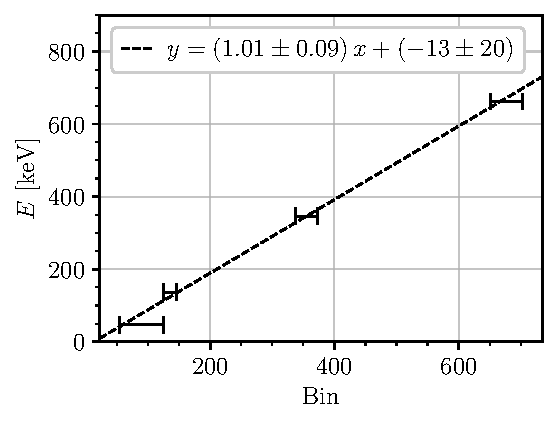
\includegraphics[scale=1]{figures/calibration_energy.pdf}
    \caption{Energy calibration of the spectrometer: known values of energies 
    versus the channel to which they were assigned by the MCA.}
    \label{fig:calibration_energy}
\end{figure}

\begin{figure}[htbp]
    \centering
    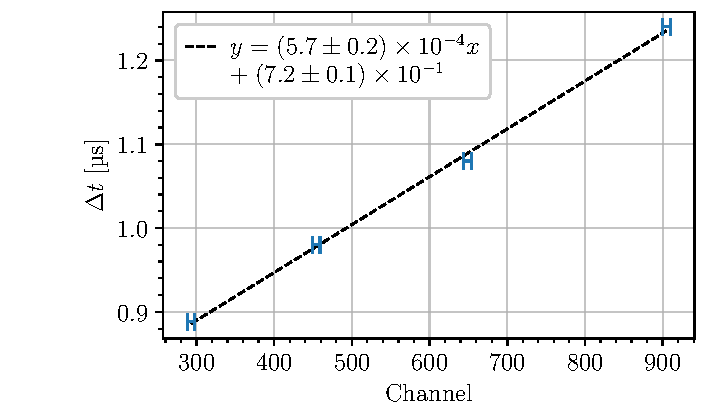
\includegraphics[scale=1]{figures/calibration_time_interval.pdf}    
    \caption{Calibration of channel to time for half-life measurement}
    \label{fig:calibration_halflife}
\end{figure}